% =============================================================================
% sections/design/drone/drone_overview.tex  -  Drone Overview
% Teams: drone (best guess - unconfirmed) / Status: EXAMPLE (scope approximation)
%
% EXAMPLE CONTENT for scope/layout approximation - not final report text.
% Adapted from the Preliminary Report's "Drone Overview" subsection, trimmed
% to minimal prose. Marked with \exampleflag on its heading in the assembler.
%
% Image is a placeholder (teams/drone/figures/drone_electronics_architecture.png,
% cropped from the Preliminary Report PDF) - swap it for an updated diagram
% by overwriting the same file.
% =============================================================================

\todo[inline]{Jury feedback (Preliminary, O/PRR-030c): the drone was never
actually shown despite an extensive description. Add real photos of the
assembled drone here, before or alongside the architecture diagram
(evidence-first rule).}

The Drone is a quadcopter built from Commercial Off-The-Shelf (COTS)
components. \autoref{fig:drone_electronics_architecture} provides a
high-level view of its onboard electronics architecture and subsystem
interfaces: the Core Avionics Subsystem, Navigation Subsystem, Perception
\& Video Subsystem, Communication Segment, and Propulsion Subsystem.

\begin{figure}[!htbp]
    \centering
    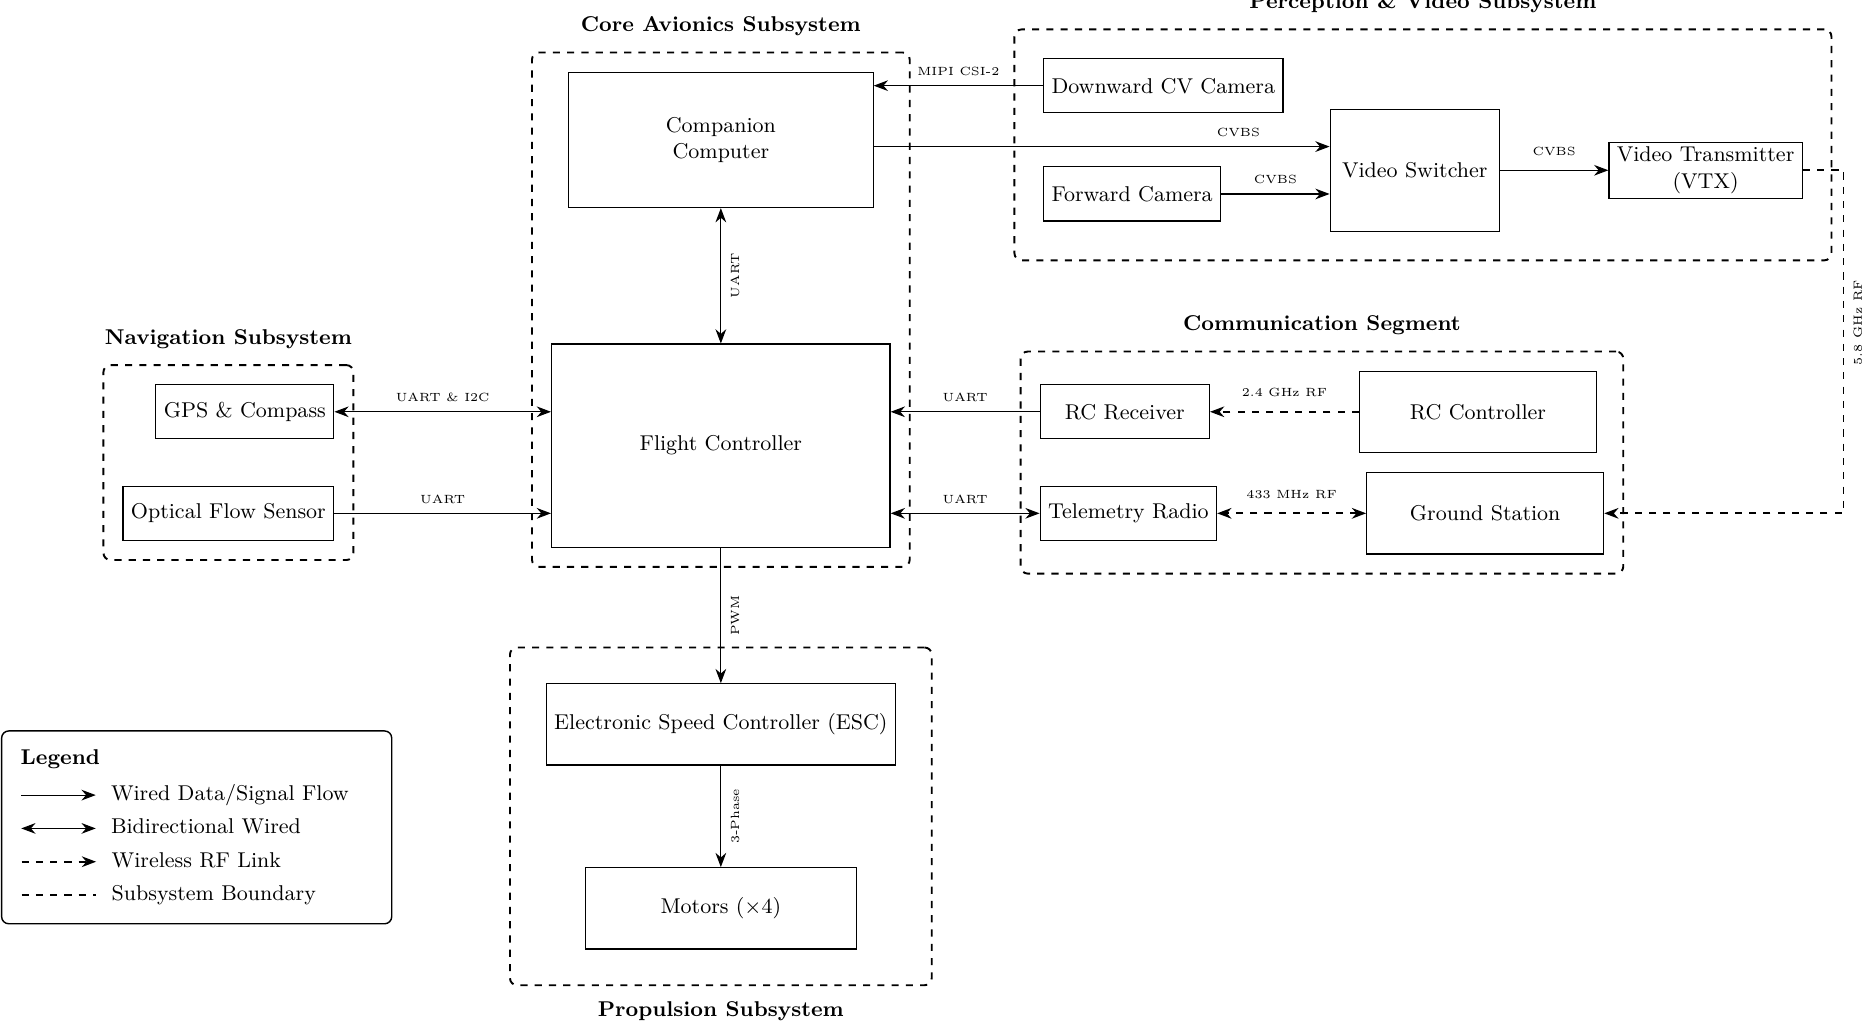
\includegraphics[width=0.85\linewidth]{teams/drone/figures/drone_electronics_architecture}
    \caption{High-level Drone electronics architecture and subsystem interfaces}
    \label{fig:drone_electronics_architecture}
\end{figure}
